\documentclass[nocrop]{bioinfo}

\copyrightyear{2020} \pubyear{2020}

\access{Advance Access Publication Date: 01 April 2020}
\appnotes{Manuscript Category}

\usepackage{enumerate}

\begin{document}
\firstpage{1}

\subtitle{RNA-Seq Clustering}

\title[A comparative study of unsupervised machine learning methods for mircoRNA sequence-based clustering]{A comparative study of unsupervised machine learning methods for mircoRNA sequence-based clustering}
\author[Samuel Acosta-Melgarejo]{Samuel Acosta-Melgarejo\,$^{\text{\sfb 1,}*}$}
\address{$^{\text{\sf 1}}$School of Biological Sciences, Faculty of Biology, Medicine and Health, The University of Manchester, Manchester, M13 9PL, UK.}

\corresp{$^\ast$To whom correspondence should be addressed.}

\history{}

\editor{}

\abstract{\textbf{Summary:} MicroRNAs are small non-coding molecules found in plants, animals and some viruses, with important functions related to post-transcriptional regulation of gene expression. The determination of microRNA families is an important task in current bioinformatics, and it largely relies on sequence-based analysis to infer and predict their properties. Computational methods from the field of machine learning had been applied to complex biological problems for a long time with excellent results, and in many occasions provided new interesting ways to conceive those problems and handle biological data. In this study we applied and assessed different unsupervised machine learning methods for microRNA clustering, using all known microRNA sequence information available in the miRBase repository. We present an overview of the different approaches used by each method, discuss their predicted families and compare the results to the real family annotations found in the database. The study shows that unsupervised machine learning approaches provide a very good tool for microRNA family prediction, and suggests that among the techniques assessed, the density-based approach used by the DBSCAN algorithm is the most suitable for microRNA clustering.\\
\textbf{Availability:} The Python-based pipeline developed for the study, miRNACluster, is publicly available at http://github.com/samuacosta/miRNACluster under the open-source GNU General Public License.\\
\textbf{Contact:} samuel.acostamelgarejo@postgrad.manchester.ac.uk\\
\textbf{Keywords:} \textit{microRNA clustering, sequence-based clustering, RNA family detection}.\\
\textbf{Word count:} 6086
}

\maketitle

\section{Introduction}

Gene expression is regulated by varied and complex mechanisms at different stages, including transcription, RNA splicing, translation, and even post-translational modification in proteins. At the post-transcriptional level, it has been established that over 60\% of human protein-coding genes are conserved targets of microRNAs, and estimations suggest that at least two-thirds of all protein-coding genes are under pressure to maintain pairing to them (Friedman et al., 2009). MicroRNAs (miRNAs) are small non-coding molecules of about 22 nucleotides, found in animals, plants and some viruses. They have roles identified in developmental timing, cell death, cell proliferation, haematopoiesis and patterning of the nervous system, and their regulatory impact is more pervasive than previously suspected (Ambros, 2004). Most of the ongoing work in miRNAs functional annotations and research is centralised in the miRBase database (Griffiths-Jones et al., 2006).

The first miRNA was discovered in 1993 during research on the development of \textit{C. elegans} (Lee et al., 1993). Since then, hundreds of other miRNAs were discovered in humans, flies and other animals, as well as in plants. A frequent challenge in the study of miRNAs is determining their "targets", or the genes that are regulated by them. This regulation is produced by the base-pairing of the miRNAs with complementary sequences in the messenger RNAs that cause the gene's expression. This causes the "silencing" of that expression. A particular miRNA can have hundreds of different messenger RNA targets, and an individual messenger RNA can be regulated by many different miRNAs (Krek et al., 2005).

The short miRNA sequences are originally derived from longer transcripts named "pri-miRNAs". These molecules are cleaved by the RNase III enzyme called \textit{Drosha} into one to six miRNA precursors ("pre-miRNAs"), hairpin loop sequences of about 70 nucleotides length. These hairpins are again processed by another RNase III enzyme called \textit{Dicer}, each one producing the actual \textasciitilde 20 nucleotide miRNA. (Li et al., 2013). In the context of miRNA sequence analysis, is frequent that the sequence used as representing the miRNA is actually the longer hairpin structure. In the miRBase dataset, the miRNAs are represented in this way.

A great effort in ongoing research is being put in determining the specific functions of miRNAs by different means. For some miRNAs such as \textit{lin-4} and \textit{let-7} there is much information about their roles and regulatory targets, but for the vast majority, the phenotypic consequences of the disruption or alteration in their regulation are not known (Bartel, 2004). One of the available pathways while researching miRNAs functions and properties is to analyse their primary structure and group them forming families. MiRNA families can be constructed following different criteria. Their meaning depends on what aspects are being taken into account, but in the context of this work, a miRNA family (or cluster) is built solely based on their nucleotide sequence similarity. The characteristics of this task make it suitable to be addressed by unsupervised machine learning methods.

Machine learning is the study of computer algorithms that improve automatically through experience (Mitchell, 1997). It is related to computational statistics, and it is considered a subset of artificial intelligence. Algorithms used in machine learning are traditionally distinguished as supervised or unsupervised, depending on the existence of a distinction between "training" data, used to prepare the algorithm in a first phase, and new data, usually consisting of a dynamic and constantly novel input. In the context of the current work, an unsupervised approach was adopted for two main reasons. As the developed pipeline was conceived as an automated alternative for family detection that could be benchmarked against the existing miRBase families, it was required that the whole dataset of existing miRNA sequences was taken into account by the clustering algorithm. Also, given the stated flexibility and complexity of the concept of a miRNA family, a distinction between training and new data does not provide the same advantages than in other applications.

A virtually infinite number of unsupervised machine learning algorithms and variants are currently being adapted, tested and assessed in many data-intensive areas. Comprehensive surveys on this type of algorithms can be found in Rui Xu and Wunsch (2005), Rokach (2010), Madhulatha (2012) and Xu and Tian (2015). In biology, as the amount and availability of data have grown exponentially in recent years, machine learning methods have been extensively applied in a wide range of areas such as genomics, proteomics, systems biology, evolution and text mining (Larra\~naga et al., 2006). In the field of sequence-based clustering, both at nucleotide and amino acid level, a great number of different machine learning algorithms have being applied and adapted for each particular case. An overview of the application of unsupervised clustering to molecular biology can be found in Nugent and Meila (2010).

There are several machine learning tools and pipelines developed specifically for miRNA clustering. Ivashchenko et al. (2016) uses a fragmented programming approach, which divides the set of sequences into independent groups, each of which will undergo a fragment clustering. Narcz et al. (2016) applies and compares four algorithms to miRNA clustering, using not only sequence information but also other types of annotations such as disease and tissue-related data to establish the families, and thus uses an intra-family quality measure to determine the compactness of the resulting families. Both of these approaches were designed to find families within partial subsets of miRNAs. Tools that were designed with the whole set of mirRNA sequences in mind are miRCluster (Wan et al., 2012), based on the K-means clustering algorithm and using the city block distance as distance measure, and miRFam (Ding et al., 2011), based on n-grams and a multiclass support vector machine, thus making it a supervised learning tool.

This project was conceived with the aim of serving as a support tool to assist with the miRNA family classification present in the miRBase database. Although the process of detecting miRNA families does not rely only on their sequence structure, an automated approach to detect these families in a draft-like fashion could greatly facilitate the process. Moreover, the comparison between clustering patterns produced by different machine learning approaches could help to adjust the existing clustering or to find new similarities among previously unrelated miRNAs. This project involved, firstly, the determination of potential unsupervised machine learning approaches and algorithm implementations that could meet the requirements imposed by the nature of the work. Furthermore, statistical validation methods that allow a relevant comparison between the performance of the different algorithms had to be determined. Additionally, an automated implementation of the research pipeline able to produce clustering information in formats akin to the ones used in the miRBase database was designed.

In this work we present miRNACluster, a Python-based pipeline for unsupervised miRNA clustering. The tool uses three different algorithms, representing different unsupervised machine learning approaches: centroid-based clustering, stochastic graph-based clustering and density-based clustering. MiRNACluster uses the entire miRBase repository of know hairpin miRNA sequences as an input, runs each algorithm and performs a statistical benchmarking using the miRBase families as ground truth class assignments. Finally, it produces an output file of families following the miRBase format and naming conventions for each algorithm. Additional raw files are optionally produced for easier sorting and cluster comparison. The statistical validation for each approach allows a cross-algorithm comparison to assess each algorithm’s suitability for miRNA sequence-based family detection.

\begin{methods}
\section{Methods}

\subsection{Data}
Version 21 of the miRBase database was used as the miRNACluster dataset. The tool uses the aliases file, containing the mappings of miRBase accession numbers with miRNA IDs for the miRBase output format, the miFam file, containing the families used as ground truth class assignments, and the hairpin FASTA file with all the miRNAs in the database to determine clustered and unclustered members.

\subsection{Environment}
MiRNACluster was written in Python version 3.7.4, and its standard libraries (Rossum, 1995), and tested on a GNU/Linux x86\_64 environment (Ubuntu Linux 18.04.4, 5.3.0-51-generic) with 16 GB of RAM and a quad-core Intel Core i7-6500U CPU at 2.50GHz. The centroid and graph-based algorithms and BLAST alignments were run though system calls to their respective binaries using the Python subprocess module.

\subsection{Algorithms}
Three different unsupervised machine learning algorithms were chosen to be part of the miRNACluster pipeline, following both computational and biological criteria. The first limitation when designing a pipeline for the whole set of known miRNAs had to do with the computational complexity of handling the dataset in memory. Both the distance matrix calculation and the clustering process itself are computationally demanding tasks. Hence, a mandatory requirement of the algorithms considered was to have been explicitly designed and tested using large datasets. Moreover, it was desirable to use algorithms representing different machine learning approaches, allowing to determine which one was more suitable for the particular case of miRNA family detection. Lastly, a desirable additional feature of the algorithms was the ability to handle highly sparse data, in the form either of a sparse distance matrix or a sparse graph. This is because the data resulting from the sequence distance measurement before clustering is more efficiently represented in this form.

\subsubsection{Centroid-based clustering}
Centroid-based clustering is one of the most popular approaches in unsupervised machine learning. A classic formulation of a centroid-based algorithm is Lloyd's algorithm (Lloyd, 1982), frequently referred to as the \textit{k-means} algorithm, has been applied and adapted for multiple tasks in many areas of biology. In this type of clustering, clusters are represented by a central vector. Providing \textit{k} is the number of desired clusters, the \textit{k-means} algorithm first finds the \textit{k} cluster centres, and then proceeds to assign the elements of the dataset to their nearest cluster centre, such that the squared distances from the cluster are minimized. Several variants exist, with differences in the values used as centres, such as \textit{k-medoids} or \textit{k-medians}, differences in the initial centres choosing, and fuzzy cluster assignments. The Clustal$\Omega$ (Sievers et al., 2011) \textit{k-means} based clustering algorithm was used in miRNACluster as the centroid-based algorithm. Clustal$\Omega$ is a multiple sequence alignment tool that combines a performance-wise implementation of distance matrix calculation with an improved version of the \textit{k-means} algorithm, \textit{k-means++} (Arthur and Vassilvitskii, 2007) in the clustering step of its multiple sequence alignment process. The \textit{k-means++} algorithm specifies an additional procedure to initialise the cluster centres at the start of the algorithm, decreasing its computational complexity. The clustering module is available as a standalone function in the full version of the software. MiRNACluster runs the GNU/Linux command line implementation of the program, in its 1.2.4 version.

\subsubsection{Stochastic graph-based clustering}
Graph clustering is another popular approach that uses network modelling to identify communities or groups with individual traits. It has been used in biology in the field of protein interaction (Bader and Hogue, 2003), epidemiology (Newman, 2003) and clustering of gene expression data (Xu et al., 2002), among others. The Markov Cluster Algorithm (Dongen et al., 2000), usually referred as the MCL algorithm, is a well-researched algorithm that follows this approach, and it has been successfully applied to protein family detection (Enright et al., 2002). This work was the basis of the additional TribeMCL Perl module, but its functionality has since been incorporated to the reference implementation of MCL. The algorithm finds clusters in graphs by a mathematical bootstrapping procedure; it uses stochastic matrices (also called Markov matrices) to model the mathematical concept of random walks on a graph. The main parameter of the algorithm is the inflation value, and it is used to increase or decrease the granularity of the clusters. The best inflation value for each context is usually empirically determined. MiRNACluster runs the reference GNU/Linux command line implementation of the algorithm (Dongen et al., 2000), in its 14-137 version.

\subsubsection{Density-based clustering}
Another seminal approach in unsupervised machine learning is density-based clustering. These algorithms represent clusters as areas of higher density within a dataset. The clusters are separated from each other by contiguous regions of low density of objects, and data objects located in low-density regions are typically considered noise or outliers (Kriegel et al., 2011). A popular algorithm using this approach is the Density-based spatial clustering of applications with noise (DBSCAN) algorithm (Ester et al., 1996). The algorithm uses two main parameters, $\varepsilon$ (the maximum distance between two points to consider them part of the same cluster) and the minimum number of elements required for a cluster. It starts from an arbitrary point, evaluates if the surrounding neighbour elements comply with the requirements set by the two parameters, and if they do, a cluster is started with them. If not, the point is taken as noise. This process is repeated until all the points are visited. A great feature of the algorithm is that it is able to use any distance function. In miRNACluster, the Scikit-Learn implementation of the DBSCAN algorithm is used (Pedregosa et al., 2011), in its 0.21.3 version.

\subsection{Distance matrix calculation}
The first step in the clustering process of all the described algorithms involves a calculation of a distance relation among all the input RNA hairpin sequences. This is usually represented with a distance matrix, a square matrix containing the pairwise distances between all the elements of the dataset. Many different approaches are used in machine learning to build distance matrices, with some algorithms built specifically to work with a particular distance measure. Given that the required memory and time for this task is proportional to $N^2$ for $N$ sequences, and that the algorithms have to cluster the whole miRBase sequence dataset, the task is computationally demanding.

\subsubsection{Embedded vectors generation (centroid-based clustering)}
For the distance matrix representation, the approach used by Clustal$\Omega$ is to use the mBed method (Blackshields et al., 2010). The method consists in embedding the sequences in a space where the similarities within a set of sequences can be closely approximated without having to compute all pair-wise distances. This embedding is done in a way that reflects the relationships between the original sequences as best as possible (Blackshields et al., 2010). Once generated, these embedded vectors are suitable to be clustered directly using the \textit{k-means} algorithm without having to represent the full distance matrix in memory at the same time. This is the default method used by Clustal$\Omega$ in its clustering module for any dataset consisting of more than 100 sequences.

\subsubsection{BLAST all-to-all sequence alignment (graph and density-based clustering)}
For graph and density-based clustering algorithms, the distance matrix is constructed from an all-to-all nucleotide sequence alignment done with the well-known Basic Local Alignment Search Tool (BLAST) (Altschul et al., 1990), using the 2.6.0+ version of the blastn binary. To avoid the computational cost of representing the dense distance matrix, the tabular ("m8") BLAST output format is used. This type of output consists of a sparse graph, a graph representation comprised of connected components that share no edges between them. This representation allows a much more performance-wise handling of the matrix. The BLAST e-values of each pair of sequences contained in the output is used as a distance measure between them. In the case of the MCL algorithm, an additional module (initially TribeMCL) has been incorporated to the reference implementation, making it able to consume the tabular BLAST output directly. For DBSCAN, some additional functionality was written in the pipeline to remove double sequence pairs and symmetrise the matrix.

\subsection{Alignment and algorithm parameters}
To adjust the BLAST all-to-all alignment to the particular case of miRNA clustering, some default alignment parameters were adjusted accordingly and validated empirically, based on the better performance of the clustering algorithms. Due to the smaller sequence length of the miRNA hairpin sequences, the word size was reduced to 7, instead of the default of 11. Additionally, the alignment's gap costs were adjusted to more stringent reward/penalty values, using the values 1 and -3, respectively, instead of the default values of 5 and -4.
The Clustal$\Omega$ avoids using a user-defined parameter of \textit{k} like is usual in most centroid-based clustering algorithms. Instead, it proceeds with a bisecting behaviour, dividing groups of sequences in two until a hard-wired cluster size threshold of 100 members is reached.

The determination of the MCL inflation value was done empirically. The inflation value regulates the granularity of the resulting clusters. It was adjusted to a value of 1.2, based on the best performance of the algorithm.

For the DBSCAN algorithm, two parameter values had to be determined. The minimum samples parameter was set to 2, following the same criteria of the miRBase clustering assignments. The $\varepsilon$ parameter regulates the algorithm coverage. If the chosen value is too small, a large part of the data will not be clustered. In the opposite case, clusters will merge and the majority of objects will be in the same cluster. The optimal value was determined empirically, on the basis of the algorithm's best performance, which was observed with an $\varepsilon$ value of $7.1 \times 10^{-5}$.

\subsection{Statistical methods}
There are several statistical functions used to benchmark the performance of unsupervised clustering algorithms, chosen depending on several factors. A frequent differentiation is made between internal and external evaluation measures, the former being based on internal cluster features such as the "compactness", and the latter on a comparison with ground truth assignments. In the context of this work, and given that the real clusters are known from miRBase, the selected functions were the Fowlkes-Mallows score and the adjusted Rand index.

\subsubsection{Fowlkes-Mallows score (FMS)}
The Fowlkes-Mallows score is a function proposed as an external similarity measure, and it is expressed as the geometric mean of the pairwise precision and recall, ignoring permutations. It is given by (1)

\begin{equation}
\text{Fowlkes-Mallows score} = \frac{\text{TP}}{\sqrt{(\text{TP} + \text{FP}) (\text{TP} + \text{FN})}}\label{eq:01}
\end{equation}
Where TP is the number of true positives (the number of pair of elements that belong to the same clusters in both true and predicted labels), FP is the number of false positives (the number of pair of elements that belong to the same clusters in the true but not in the predicted labels) and FN is the number of false negatives (the number of pair of elements that belongs in the same clusters in the predicted but not in the true labels) (Fowlkes and Mallows, 1983). The score has a bounded range of [0, 1], where 0 indicates purely independent labellings and 1 the perfect match score.

\subsubsection{Adjusted Rand index (ARI)}
The Rand index is a similar external similarity measure function proposed in Rand (1971) for an objective measure of the similarity of two clustering assignments when truth values are known. It is given by (2).

\begin{equation}
\text{Rand Index (RI)} = \frac{a + b}{C_2^{n_{samples}}}\label{eq:02}
\end{equation}
Where $a$ is the number of pairs of elements that are in the same set in the ground truth assignments and in the same set in the assessed clustering, $b$ is the number of pairs of elements that are in different sets in the ground truth assignments and in different sets in the assessed clustering, and \(C_2^{n_{samples}}\) is the total number of possible pairs.

It was adjusted for chance normalisation in Hubert and Arabie (1985), and this version is widely used for unsupervised clustering evaluation. The adjusted version is given by (3).

\begin{equation}
\text{Adjusted Rand Index (ARI)} = \frac{\text{RI} - E[\text{RI}]}{\max(\text{RI}) - E[\text{RI}]}\label{eq:03}
\end{equation}
Where $E[\text{RI}]$ is the expected index of random labellings. The ARI has a bounded range of [-1, 1], where negative values indicate independent labellings, and a value of 1 is the perfect match score.

The functions' formalisations were adapted from the Scikit-Learn user guide (Devs, 2019)

\subsection{True-predicted cluster equivalence}
When using external validation methods to compare different clustering approaches, a particular requirement is to establish the identity of the clusters. The criteria used to find the equivalent clusters may vary depending on the particular situation. In some contexts, particular cluster element or elements can be used to identify a certain cluster. Within sequence-based clustering, the cluster comparison must be done taking into account all the members of the cluster. For this purpose, a confusion matrix calculation was implemented in the pipeline. This allows matching real with predicted clusters based on the number of shared element memberships. Clusters are matched on a one-to-one basis, and unmatched clusters are added as new families.

\end{methods}

\section{Results and discussion}

\subsection{Dataset coverage and cluster sizes}
The three algorithms showed different levels of coverage of the dataset. MiRBase has a total of 28645 miRNA hairpin sequences, with 19906 of them grouped in 1983 identified miRNA families with at least two sequences. That represents a 69.49\% of dataset coverage, and the average number of miRNAs per 2+ cluster is 10.04.
%---------------------------
\begin{figure}[ht]
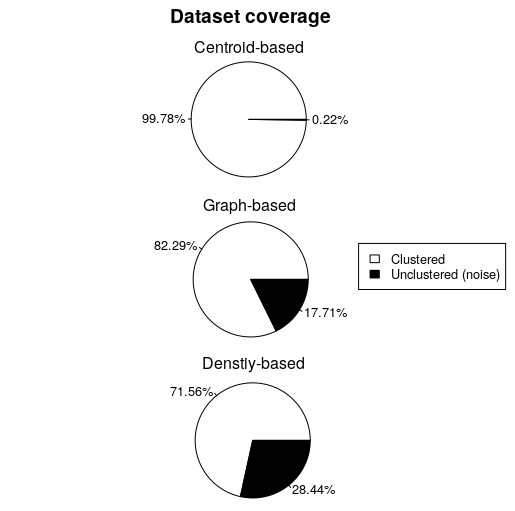
\includegraphics[scale=0.45]{img/coverage.png}
\caption{Data coverage patterns of each algorithm. A very high coverage value suggests higher sensibility to noise data.}\label{fig:01}
\end{figure}
%---------------------------
The algorithms showed very variable coverage patterns (Fig 1). The Clustal$\Omega$ algorithm showed the most different coverage values, compared to miRBase and to the other algorithms. Almost the whole dataset was clustered, the coverage value being determined at 99.78\%, with 28583 clustered and 10 unclustered sequences. The total number of 2+ clusters found was 667 and the average number of miRNAs per cluster was 42.85. The MCL algorithm grouped 23573 miRNAs in 2253 different clusters, with 5071 sequences labelled as noise, covering 82.29\% of the dataset. The average number of sequences per cluster was 10.46. The DBSCAN algorithm clustered 20501 sequences in 2192 clusters, achieving 71.56\% coverage (8143 sequences labelled as noise). The average number of miRNAs per cluster was 9.35.

\subsection{Statistical validation}
Despite having different bounded ranges, both the Fowlkes-Mallows score and the adjusted Rand index had similar values throughout the statistical assessment of the algorithms. The Fowlkes-Mallows score tended to evaluate the clusterings in a slightly more positive way (Fig. 2).
%---------------------------
\begin{figure}[ht]
\centering
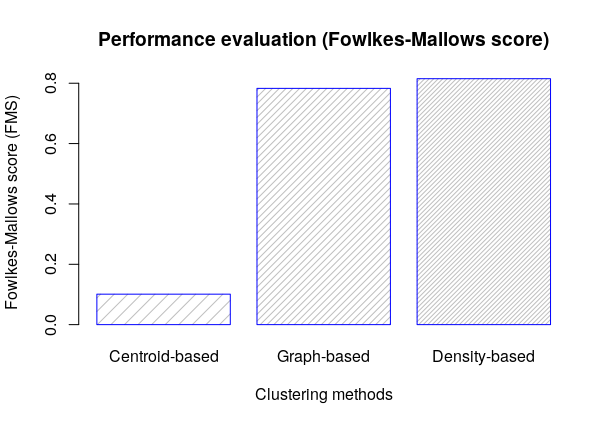
\includegraphics[scale=0.45]{img/fms.png}
\caption{FMS quality values for each algorithm.}\label{fig:02}
\end{figure}
%---------------------------

In the clustering similarity evaluation, the ClustalΩ algorithm also showed a differentiated behaviour. Both measures had the lowest values among the three algorithms, showing a clear difference from the ground class assignments. Its value for the FMS was 0.101, which is very close to the independent labelling score, and in this context they can be considered very poor. In a different vein, the other two algorithms showed a very good performance, with values of 0.783 for the graph-based algorithm and 0.815 for the density-based algorithm, which was the best quality value overall. 
%---------------------------
\begin{figure}[ht]
\centering
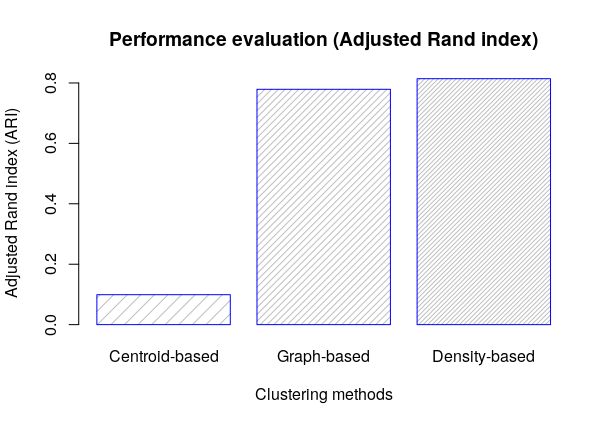
\includegraphics[scale=0.45]{img/ari.png}
\caption{ARI quality values, lower on average.}\label{fig:03}
\end{figure}
%---------------------------

Similar quality assignments are observed with the adjusted Rand index (Fig. 3). The centroid-based algorithm had the lowest score overall with this measure, with a value of 0.099. The MCL algorithm achieved a value of 0.779 and the DBSCAN algorithm, 0.814. Both quality measures point to the DBSCAN density-based algorithm as having the best performance.

\subsection{Clustering overview}
It is very clear from the results that the clustering produced by the centroid-based algorithm used by Clustal$\Omega$ differs a lot from the families identified in miRBase. Based on the statistical results and studying the different clusters produced by the algorithm, it seems clear that one of the causes of this difference is the hard-wired cluster size threshold used in the Clustal$\Omega$ algorithm. More than 30 families in miRBase currently have a cluster size above that threshold, and some have many more sequences. Moreover, the algorithm has a very high sensitivity to noise, producing a very high coverage of the dataset at the cost of having clusters with too many false positives, which is typically not desirable when clustering biological data. A potentially better result may be obtained avoiding the use of embedded vectors during the similarity matrix calculation, but the fact that the cluster size threshold is not modifiable in the current implementation of the Clustal$\Omega$ algorithm makes it impossible to take advantage of the better similarity computation. The explanation of this limitation in the algorithm implementation is that it was conceived primarily to produce clusterings that are particularly useful for the construction of UPGMA guide trees used in the Clustal$\Omega$ multiple sequence alignment process. But putting aside this limitation, the algorithm's difficulty to deal with noise elements makes it very difficult to be adapted to the context of miRNA clustering.

On the other hand, the graph and density-based algorithms performed very well. A possible explanation of their good performance is that both algorithms were designed with very sparse data in mind, shown in their ability to cluster over sparse graphs, such as the sequence distance matrix produced by multiple sequence alignment. The suitability of the MCL algorithm to handle biological data has been previously demonstrated in the field of protein family detection, and we found that its application to nucleotide-based sequences is equally successful, both with small and large clusters. A great advantage of this algorithm in this context is the cluster granularity customisation. Determining the value of the optimal inflation parameter can be challenging on some applications, but due to existence of reference values in this work, it allows to tune the clustering pattern accordingly, which is not possible with the centroid-based algorithm. In terms of usability, the algorithm implementation produces the most straightforward output format among the algorithms tested, with a very easily parseable syntax. The MCL algorithm produces a slightly higher number of clusters and has better coverage than DBSCAN, but the statistical similarity methods show that the latter gets a bit closer to the miRBase assignments. The DBSCAN also has the advantage of being flexible enough to adapt it to the working context. However, the regulation is performed in a slightly different way. The $\varepsilon$ value used by the DBSCAN algorithm not only regulates the granularity of the clusters, but it was found that it has a greater impact on the detection of noise. Given that the miRBase assignments exhibit a considerable amount of unclustered sequences, better noise detection is a desirable feature of the algorithm, and it is likely to be the reason of the better performance of DBSCAN compared to MCL. The output produced by DBSCAN requires slightly more effort to produce readable information.

Examining particular miRNA families, we found some similarities as well as differences in the way both algorithms perform the clustering. The two most populous miRNA families in the miRBase dataset are the \textit{let-7} and \textit{mir-10} families. The \textit{let-7} family is identified by \textit{lethal-7}, one of the first two known miRNAs, and it is very well known and annotated. Both MCL and DBSCAN detected the cluster in a very similar way, dividing it into one main cluster of about 400 miRNAs and two extra clusters with two miRNAs each. Their clustering differed more with the \textit{mir-10}, MCL using only two clusters and DBSCAN, five.

\subsection{The miRNACluster tool}
The miRNACluster Python pipeline built for this project integrates all the steps necessary to read the miRBase input files, run all the algorithms and obtain the statistical information from them in one execution. It also generates several output files to browse and compare the generated families.

\subsubsection{Performance}
MiRNACluster was developed with the whole miRBase sequence dataset in mind, so it uses system calls to installed binaries whenever possible to accelerate the process. The two most computationally demanding tasks in the pipeline are the Clustal$\Omega$ distance matrix calculation and clustering and the BLAST all-to-all alignment. An approximate estimate of the execution time of the complete pipeline surpasses the 2.5-hour mark. MiRNACluster implements a cache parameter that allows to use existing generated files and avoid certain steps in the pipeline. Possible values are \textit{formatdb} (BLAST-formatted database creation from the hairpin file), \textit{blast} (BLAST all-to-all alignment), \textit{clustal} (Clustal$\Omega$ clustering file generation), \textit{mcl} (MCL clustering file generation). 

\subsubsection{Input and output structure}
The tool takes the miRBase \textit{miFam.dat}, \textit{hairpin.fa} and \textit{aliases.txt} files from \textit{input/} directory and creates several ouput files in the \textit{output/} directory. The main three files are named \textit{miFamCentroid.dat}, \textit{miFamGraph.dat} and \textit{miFamDensity.dat}, and correspond to the clustering generated by each algorithm. The files follow the format of the \textit{miFam.dat} file. The clusters are identified by IDs inferred from its members following a convention almost identical to the one used by miRBase, and they are assigned a sequential accession number. Additional simplified "raw" files that facilitate comparison are generated for each algorithm and for the miRBase \textit{.dat} file, using the \textit{\_byname}, \textit{\_bysize}, and \textit{\_labelsonly} suffixes for files ordered by cluster name, size, and with only cluster labels, respectively. A file with the \textit{\_equivalences} suffix is generated to show the true-predicted cluster mappings used for that particular algorithm. Intermediate "cache" files are also generated for BLAST database formatting and alignment, Clustal$\Omega$ algorithm output and MCL algorithm output. The clustering statistical information is displayed through the standard output.

\section{Conclusion}
In this work, we have addressed and evaluated the suitability of unsupervised machine learning methods to the problem of miRNA sequence-based family detection. Three very different algorithms were chosen to represent different approaches within machine learning, and they were compared against the miRBase classification to evaluate their accuracy. Two of those approaches, stochastic graph-based clustering and density-based clustering have shown very promising results for the task at hand. Additionally, a standalone automated tool was created for the project, making the results easy to replicate and providing a complete pipeline that can be used as an aid for miRNA family detection to complement, adjust or improve the cluster predictions found in the miRBase database.

The results of this work can be assessed in the light of two previous efforts in the literature that share similar goals. The miRCluster tool was designed to use the complete miRBase dataset for analysis, although it assesses its results creating three different partial datasets from two different versions of miRBase. It is stated that the reason for this that it reflects their specific research motivations, which were the study of feature selection test, new family evaluation and novel family discovery from unclassified miRNAs. Moreover, the study explicitly excludes animal and plant families that contain less than four members. Although the software is not available anymore in executable or source form, the report describes the generation of interesting information statistical information from the generated clusters. The results are assessed using the F-measure, a test accuracy metric, although it is presented separately for each partial dataset. Compared to miRCluster, advantages of miRNACluster are that it operates with the complete miRBase dataset, which allows for more precise comparison of the algorithms' results to the real families, and that more than one alternative is offered as clustering method. The use of the F-measure as quality metric between clusters has been criticised in some respects (Hand and Christen, 2018). The method chosen by miRCluster is a standard \textit{k-means} algorithm with the city block distance as a distance measure, chosen after empirical test. We understand that this is not the best approach, because the \textit{k-means} algorithm was designed specifically to operate with the Euclidean distance. Additionally, having included a similar centroid-based algorithm in the current work, it showed strong limitations in its statistical assessments and its handling of noise. This limitation was also identified and addressed in the miRCluster paper.

The miRFam tool is another tool developed with objectives similar to those of miRNACluster. It is reported to have very high accuracy values and also a very good performance even with big datasets. It is reported that the tool was tested with the complete dataset of the version 15 of the miRBase dataset, but similarly to miRCluster, for most of its measurements exclude some families from the comparison, in this case clusters with less than five members. The software is still available as source code, although it is developed only for Windows environments up to Windows 7 and involves a somewhat complex compilation process, having being developed in C++. The main difference between the approach used in miRFam and the one in miRNACluster is that miRFam addressed the problem applying supervised learning. It uses multiclass support vector machines (SVMs), a set of machine learning methods frequently used for classification, regression and outliers detection. This means, among other things, that in order for the algorithm to work, the dataset has to be divided in training and testing data, in a typical supervised learning fashion. In the miRNA families classification context, this has the disadvantage of making the clustering highly dependent on the structure of the clusters elected as part of the training set, which greatly limits the classification accuracy. This problem was addressed in the miRFam paper, and the adaptation of their approach to use an unsupervised method is mentioned as an issue for future work.

Overall, it can be said that the project produced very satisfying and promising results, both in terms of the analysis of the data and its statistical validation and of the supporting tool developed. Some limitations arose from the particular requirement of having to deal with a big dataset, which led to less algorithmic approaches to explore for the task. Moreover, the decision of implementing the pipeline in Python, despite having the advantages of producing software that is comparatively easy to run and test in several environments, also makes the tool to be in disadvantage in performance compared to more low-level, compiled implementations such as the one that miRFam has. Additionally, future important improvements to the tool would be to create an automated dependency installation script for different platforms and, better still, its adaptation for deployment as a web service with the capacity to work directly with the miRBase online repository. Lastly, an important aspect for future work is to make it easier for miRNACluster to operate with more limited subsets of miRNA sequences and analyse its accuracy in more specific biological contexts.

\section{Acknowledgements}
This work was done with the support of the SGJlab at the School of Biological Sciences facilities of the University of Manchester, under the supervision of Dr Sam Griffiths-Jones, for whose guidance I am immensely grateful. The project was part of the Bioinformatics and Systems Biology master's programme, for which I was sponsored by Chevening Scholarships, the UK government's global scholarship programme, funded by the Foreign and Commonwealth Office (FCO) and partner organisations.

\textit{Conflict of interest:} None declared.

\section{Declaration}
The content of this paper is the author's original work unless referenced clearly to the contrary, and no portion of the work referred to in it has been submitted in support of an application for another degree or qualification of this or any other university or other institute of learning.

\section{Intellectual property statement}
\begin{enumerate}[i. ]

\item  The author of this paper (including any appendices and/or schedules to this paper) owns certain copyright or related rights in it (the "Copyright") and s/he has given The University of Manchester certain rights to use such Copyright, including for administrative purposes.

\item Copies of this paper, either in full or in extracts and whether in hard or electronic copy, may be made only in accordance with the Copyright, Designs and Patents Act 1988 (as amended) and regulations issued under it or, where appropriate, in accordance with licensing agreements which the University has entered into. This page must form part of any such copies made. 

\item The ownership of certain Copyright, patents, designs, trademarks and other intellectual property (the "Intellectual Property") and any reproductions of copyright works in the paper, for example graphs and tables ("Reproductions"), which may be described in this paper, may not be owned by the author and may be owned by third parties. Such Intellectual Property and Reproductions cannot and must not be made available for use without the prior written permission of the owner(s) of the relevant Intellectual Property and/or Reproductions.

\item Further information on the conditions under which disclosure, publication and commercialisation of this paper, the Copyright and any Intellectual Property and/or Reproductions described in it may take place is available in the University IP Policy, in any relevant Paper restriction declarations deposited in the University Library, and The University Library's regulations.

\end{enumerate}

%\enlargethispage{6pt}

\bibliographystyle{plainnat}
\nocite{*}
\bibliography{ref}


\end{document}
